% Erzeugung des Dokuments als standalone, andernfalls kann der TikZ-Code nicht kompiliert werden!
\documentclass{standalone}

% Einige Packages, die nützlich sind für die Erstellung von Grafiken:
\usepackage[utf8]{inputenc}
\usepackage{soulutf8}
\usepackage{pgfplots}
\usetikzlibrary{plotmarks}

% Für das Einbinden von Tabellen in Bilder können diese Packages hilfreich sein:
\usepackage{harveyBalls}
\usepackage{fontawesome}
\usepackage{multirow}

\begin{document}

	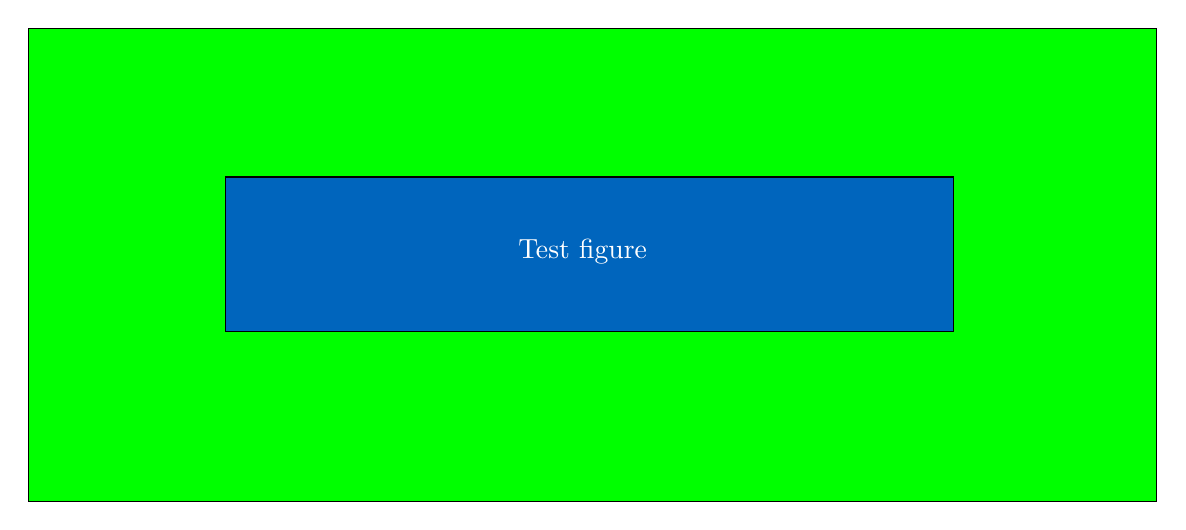
\begin{tikzpicture}[x=0.75pt,y=0.75pt,yscale=-1,xscale=1]
		
		% Shape: großes, grünes Rechteck
		\draw  [fill={rgb, 255:red, 0; green, 255; blue, 0 } ,fill opacity=1 ] (72,27) -- (615.8,27) -- (615.8,254.9) -- (72,254.9) -- cycle ;
		
		% Shape: kleineres, blaues Rechteck
		\draw  [fill={rgb, 255:red, 0; green, 101; blue, 189 } ,fill opacity=1 ] (166.9,98.7) -- (517.8,98.7) -- (517.8,173) -- (166.9,173) -- cycle ;
		
		% Text box
		\draw (306.85,127.35) node [anchor=north west][inner sep=0.75pt] [color={rgb, 255:red, 255; green, 255; blue, 255 }  ,opacity=1 ] [align=left] {Test figure};
		
	\end{tikzpicture}

\end{document}